%%%%%%%%%%%%%%%%%%%%%%%%%%%%%%%%%%%%%%%%%
% Stylish Article
% LaTeX Template
% Version 2.1 (1/10/15)
%
% This template has been downloaded from:
% http://www.LaTeXTemplates.com
%
% Original author:
% Mathias Legrand (legrand.mathias@gmail.com) 
% With extensive modifications by:
% Vel (vel@latextemplates.com)
%
% License:
% CC BY-NC-SA 3.0 (http://creativecommons.org/licenses/by-nc-sa/3.0/)
% 
%%%%%%%%%%%%%%%%%%%%%%%%%%%%%%%%%%%%%%%%%

%----------------------------------------------------------------------------------------
%	PACKAGES AND OTHER DOCUMENT CONFIGURATIONS
%----------------------------------------------------------------------------------------

\documentclass[fleqn,10pt]{SelfArx} % Document font size and equations flushed left

\usepackage[english]{babel} % Specify a different language here - english by default

\usepackage{lipsum} % Required to insert dummy text. To be removed otherwise

\usepackage{tikz}
\usepackage{todonotes}
\usepackage{multicol}

\usepackage{listings} % Required for inserting code snippets

%Changing lis name from 'Listing' to 'Code Example'
\renewcommand{\lstlistingname}{Code Example}

%Defining colors used in our style
\definecolor{color3}{RGB}{230, 231, 231} % background
\definecolor{Blue}{RGB}{0, 51, 204} % keywords
\definecolor{Gray}{RGB}{153, 153, 153} % line numbers
\definecolor{PineGlade}{RGB}{204, 204, 153}

%Our style
\lstdefinestyle{Python1}{ 
language=Python,
frame=single,
basicstyle=\scriptsize\ttfamily,
backgroundcolor=\color{color3},
keywordstyle=\color{color1}\bf,
captionpos=b,
breakatwhitespace=false,
breaklines=true,
numbers=left, % Location of line numbers, can take the values of: none, left, right
numbersep=6pt, % Distance of line numbers from the code box
numberstyle=\tiny, % Style used for line numbers \color{Gray}
commentstyle=\usefont{T1}{pcr}{m}{sl}\color{color1}
} 

\newcommand{\insertcodefile}[2]{\lstinputlisting[caption=#2,label=#1,style=Python1,float=h,belowskip=-0.8\baselineskip]{codeRelated/scripts/#1}} % The first argument is the script location/filename and the second is a caption for the code

\newcommand{\insertcodefileline}[4]{\begin{itemize}\item[]\lstinputlisting[firstnumber=#3,firstline=#3,lastline=#4,caption=#2,label=#1,style=Python1]{codeRelated/scripts/#1}\end{itemize}}

%----------------------------------------------------------------------------------------
%ALDRIG KALD DENNE STYLE!!!!!!!!!!!!!!!!!!!!!, kun her som reference til hvordan vi laver vores egen.
%----------------------------------------------------------------------------------------

\lstdefinestyle{Style1}{ % Define a style for your code snippet, multiple definitions can be made if, for example, you wish to insert multiple code snippets using different programming languages into one document
language=Python, % Detects keywords, comments, strings, functions, etc for the language specified
backgroundcolor=\color{highlight}, % Set the background color for the snippet - useful for highlighting
basicstyle=\footnotesize\ttfamily, % The default font size and style of the code
breakatwhitespace=false, % If true, only allows line breaks at white space
breaklines=true, % Automatic line breaking (prevents code from protruding outside the box)
captionpos=b, % Sets the caption position: b for bottom; t for top
commentstyle=\usefont{T1}{pcr}{m}{sl}\color{DarkGreen}, % Style of comments within the code - dark green courier font
deletekeywords={}, % If you want to delete any keywords from the current language separate them by commas
%escapeinside={\%}, % This allows you to escape to LaTeX using the character in the bracket
%firstnumber=1, % Line numbers begin at line 1
frame=single, % Frame around the code box, value can be: none, leftline, topline, bottomline, lines, single, shadowbox
frameround=tttt, % Rounds the corners of the frame for the top left, top right, bottom left and bottom right positions
keywordstyle=\color{Blue}\bf, % Functions are bold and blue
morekeywords={}, % Add any functions no included by default here separated by commas
numbers=left, % Location of line numbers, can take the values of: none, left, right
numbersep=10pt, % Distance of line numbers from the code box
numberstyle=\tiny\color{Gray}, % Style used for line numbers
rulecolor=\color{black}, % Frame border color
showstringspaces=false, % Don't put marks in string spaces
showtabs=false, % Display tabs in the code as lines
stepnumber=1, % The step distance between line numbers, i.e. how often will lines be numbered
stringstyle=\color{Purple}, % Strings are purple
tabsize=2, % Number of spaces per tab in the code
}
 %Everything related to making the code examples look oh so pretty
%\usepackage{listings}

\usepackage{hyperref}

\usepackage{cleveref}


%----------------------------------------------------------------------------------------
%	COLUMNS
%----------------------------------------------------------------------------------------

\setlength{\columnsep}{0.55cm} % Distance between the two columns of text
\setlength{\fboxrule}{0.75pt} % Width of the border around the abstract

%----------------------------------------------------------------------------------------
%	COLORS
%----------------------------------------------------------------------------------------

\definecolor{color1}{RGB}{0,0,90} % Color of the article title and sections
\definecolor{color2}{RGB}{0,20,20} % Color of the boxes behind the abstract and headings

%----------------------------------------------------------------------------------------
%	HYPERLINKS
%----------------------------------------------------------------------------------------

\usepackage{hyperref} % Required for hyperlinks
\hypersetup{hidelinks,colorlinks,breaklinks=true,urlcolor=color2,citecolor=color1,linkcolor=color1,bookmarksopen=false,pdftitle={Title},pdfauthor={Author}}

%----------------------------------------------------------------------------------------
%	CUSTOM COMMANDS
%----------------------------------------------------------------------------------------

\newcommand{\FW}{TestFramework}

%----------------------------------------------------------------------------------------
%	ARTICLE INFORMATION
%----------------------------------------------------------------------------------------

\JournalInfo{This is the journal info} % Journal information
\Archive{This is actually additional notes} % Additional notes (e.g. copyright, DOI, review/research article)

\PaperTitle{Testing of ETL} % Article title

\Authors{Alexander Brandborg\textsuperscript{1}, Mathias Claus Jensen\textsuperscript{1}, Mikael Vind Mikkelsen\textsuperscript{1}, Arash Michael Sami Kjær\textsuperscript{1}} % Authors
\affiliation{\textsuperscript{1}\textit{Student at the Department of Computer Science, Aalborg University, Aalborg, Denmark}} % Author affiliation
%\affiliation{\textsuperscript{2}\textit{Department of Chemistry, University of Examples, London, United Kingdom}} % Author affiliation
%\affiliation{*\textbf{Corresponding author}: john@smith.com} % Corresponding author

\Keywords{Datawarehouse --- ETL --- Testing} % Keywords - if you don't want any simply remove all the text between the curly brackets
\newcommand{\keywordname}{Keywords} % Defines the keywords heading name

%----------------------------------------------------------------------------------------
%	ABSTRACT
%----------------------------------------------------------------------------------------

\Abstract{The python package pygrametl allows developers to construct ETL systems through an API. We develop a testing framework, \FW{}, which allows testers to evaluate programs developed using pygrametl. The framework is developed for both functional- and regression testing at the system level. It is based on source to target testing. Here an ETL system is tested by asserting about properties of the DW, which it populates. \FW{} can be used to check whether assertions are upheld by such a DW. These assertions are implemented using \FW{}’s predicate classes. These allow testers to assert about DW properties relating to data loss and business rules. After development we evaluate \FW{} against manual testing, where testers write SQL to test for properties. We found that both methods result in test implementations with the same runtime. However, manual testing needed 110 statements for its implementation, where \FW{} only needed 11.}

%----------------------------------------------------------------------------------------

\begin{document}
\lstset{language=Python}

\flushbottom % Makes all text pages the same height

\maketitle % Print the title and abstract box

\thispagestyle{empty} % Removes page numbering from the first page

%----------------------------------------------------------------------------------------
%	ARTICLE CONTENTS
%----------------------------------------------------------------------------------------

\section{Introduction}\label{intro} % The \section*{} command stops section numbering
%\addcontentsline{toc}{section}{Introduction} % Adds this section to the table of contents
To make sure that a piece of software can be expected to run at low risk of failure, it must be tested. Today we have specialized software that assist in the automatic execution of tests. This allows testers to focus more on what to test and less on test implementation. Conceptually this should lead to tests of a higher quality.

Some testing tools such as JUnit have a broad application, while other test frameworks have a more specific use. Per extension, there exists many tools exclusively used for testing Extract-Transform-Load (ETL) systems. These systems support the creation and update of data warehouses (DW), which are mainly used for business analysis. An ETL process will extract data from a set of sources, apply transformations to that data and then load it into a DW. Often GUI-based tools are used, when developing ETL systems. The pygrametl python package, which is open source, allows for coding entire ETL systems instead. The idea being that experts perform better when using an API rather than a GUI \cite{thomsen2009pygrametl}. Our goal for this article is to develop a testing framework, which may assist users of pygrametl in testing their ETL systems.

ETL testing may be set up manually using SQL. Yet, in the current market many different testing tools exists. These allow for the automation of tests. Testing often occurs by focusing on the DW, which the ETL system populates. QuerySurge\cite{QuerySurge} for example, focuses on comparing the data from sources to the data in the DW. The tool is build on the idea that data is often unaltered, as it passes through the ETL process. This means that column A in a source must be one-to-one mappable to column B in the DW. Testing of this type only requires the user to supply some simple mappings between sources and DW. As such, QuerySurge presents itself as novice-friendly and allows for testing through a GUI. Yet, if mappings between source data and DW become more complex, testers will need to write up some SQL code. We determine that this kind of tool is not fitting for the users of pygrametl. As pygrametl users are experts, they will not gain anything from the novice-friendly features of QuerySurge. The amount of code needed for testing may also be rather large, if there is a frequent need for writing SQL.

Testing may also occur through the comparison of tables within a populated DW to those defined by the user. By writing up a table, testers assert, how they expect a DW table to look after load. The truth value of this assertion can be found by comparing to the actual DW table. For this, tools such as AnyDBTest\cite{AnyDbTest} may be used. AnyDBTest also allows testers to describe, what kind of comparison should be made. For example, we may test that one table is the subset of another. Our issue with this type of testing requires the setup of many user-defined tables. Again a large amount of test code needs to be written. We do however believe that table comparison is a powerful tool for ETL testing. Yet, comparison between tables should not be the only assertable property of a DW.

Having looked at some of the currently available tools, we find that they require a lot of test code to be written. To get a wider test coverage, we need to decrease the amount of code necessary for each test. We also fear that faults may be more likely to occur in the test code, as it grows larger. Such faults can undermine the usefulness and accuracy of test results.

To allow for automated testing of pygrametl programs, we have developed \FW{}. Like AnyDBTest it is assertion-based. However, it does not only allow for assertions to be made upon the relationships of tables. Assertions may relate to other DW properties such as data integrity. The framework allows for functional testing at the system level, once all components of the ETL have been integrated. As the framework automates test execution, it can also be used for regression testing. We aim to help testers in writing less code for a single test. This should lead to less time spend on each test, enabling a wider coverage during testing. Covering more of the software should increase its overall quality. We also need for the tests to be executed at a reasonable speed. If the tests are quick to write, but slow to execute, users may fall back on other tools or perform testing manually.

The rest of this paper is organized as follows. \Cref{sect:RelatedWorks} will give a brief overview of some related literature. This is followed by an introduction to the pygrametl python package in \cref{sect:pygrametl}. \Cref{sect:btesting} will explain some basic testing terminology relevant to the paper. This leads into an overview of \FW{} in \cref{sect:Overview}, followed by some sections describing its implementation. \Cref{sec:dwpopulator} shows how the framework allows for dynamic replacement of sources and DW in a pygrametl program.  In \cref{sect:interdatarep} we describe the classes used to represent the DW during testing. Afterwards, \cref{sect:pred} explains the different types of predicates, used to assert properties of a DW. After implementation \cref{sect:eval} will focus on evaluating the framework. Finally, in \cref{sect:conc} we conclude upon the framework.



\section{pygrametl}\label{sect:pygrametl}
In this section we give a quick outline of the python package pygrametl, as \FW{} works in combination with this. The section is based upon the pygrametl documentation and its source code\cite{pygramSource}.

The package was developed at Aalborg University in Denmark and was released as open source in 2009. It has found use in a range of different systems since then. It was developed to let users develop ETL programs by coding in python. This stands in contrast to other products on market, which mainly allow for ETL development through a GUI. By allowing expert developers to use an API instead, it is believed that some might be more productive.

pygrametl provides assistance for the implementation of all three parts of an ETL system. Classes in the datasources.py module allow for the extraction of data from sources. A source may either be a CSV file or an SQL database. Data is always extracted as dictionaries. Each dictionary corresponds to a row from the source, and each key-value pair matches an attribute-value pair of that row. Transformation of the extracted data is supported by the classes found in steps.py. Although users often perform their transformations through normal python. Afterwards, loading is performed using the connectionwrapper class found in init.py and the classes found in tables.py. A connectionwrapper object is used as the default connection to the DW that must be populated. The table.py classes support the use of different types of dimension and fact tables. Once a table class is instantiated it is associated with an actual table in the DW. It can then be used to load data into that table.

Note that pygrametl never sets up sources or DW, it merely provides a way to work with them at an abstract level. These need to be set up separately by developers, and pygrametl must be used in conjunction with a python module that can access them. Such modules are often developed to be used with a specific Database management systems (DBMS). However, pygrametl only works with modules that conform to the PEP249 standard \cite{pep249}. This standard encourages similarity between modules that access databases. Because of this, pygrametl works with a broad range of DBMS's. To access databases, pygrametl generates SQL code dynamically. The SQL generated is not DBMS specific and uses only standard keywords such as UPDATE,SELECT and JOIN. This is done to ensure compability with the different PEP249 modules and their related DBMSs. \FW{} aims for the same compatibility and avoids more DBMS specific syntax and functionality when generating SQL code. This also makes accessing meta data on a database or table difficult, as PEP249 does not enforce a standard way to do this.
\section{The Basics of Software Testing}\label{sect:btesting}
This section introduces some of the basics of software testing. These will assist in understanding the work documented in later sections. The definitions used in this section are taken from the books textit{Guide to Advanced Software Testing} by Anne Mette Jonassen Hass\cite{Hass} and \textit{Software Testing Techniques} by Boris Beizer\cite{Beizer}.

Testing is an integral part of the software development process at large. It is included in many different software process models. But, what is testing exactly? Hass defines it as follows: 
 \begin{quotation} \textit{Testing gathers information about the quality of the object under test.}\end{quotation}  
Knowing the quality of a piece of software allows an organization to evaluate, whether it is fit for purpose. If not, test results may guide an effort to increase quality.

Before tests can be executed they must be designed.  Design can be done from two different points of view: Functional and Structural. With functional, software is treated like a black box receiving input and computing output. Tests are designed to verify, whether the software conforms to specified behavior. Structural involves designing based on the internal structure of the software. Here a tester could for instance test how a piece of code logically branches during execution. The structural approach is often used, when testing individual components. Functional is more apt to use, when testing a set of integrated units or an entire system. 

As with any other process, testing is restricted by both time and resources available. These greatly affect the quality of testing performed, often called test coverage. Because of this, testers are almost never able to perform exhaustive testing, where all combinations of input and preconditions are tested. Instead, testers select the most important areas to focus on during testing.  

Tools are often used to assist in the testing process. An example is the testing framework, which assist in the automatic execution of tests. By the push of a button, a framework can execute a set of user-defined test cases, setting up and tearing down objects as needed. A test case is a well defined set of preconditions and input given to a component. This is  accompanied by a set of expected output and postconditions. A test case passes or fails, depending whether actual output and postconditions match expectations.  The required test coverage is often acquired by designing a set of test cases. An advantage of frameworks is that testers can spend more time on test design. Less time will have to be spend on how to implement tests.  In theory this leads totesting of a higher quality.

Another bonus of using a framework is that it allows for regression testing. This becomes mostly relevant in the maintenance part of the software life cycle. During this time, new features may be added and bugs fixed. Testers want to ensure that such changes do not lead to regression,  where software quality deteriorates. With a framework, regression testing is simple. Once a set of test cases have been set up, they can be run after a change has been made. This will then  gauge whether regression has occurred.



\section{Overview of \FW{}}
In this section we will give an overview of \FW{} and its major components. The following sections will go into detail about each individual part of the framework.

The purpose of \FW{} is to assist in functional source to target testing of ETL programs developed using pygrametl. As such, testing is performed by asserting about properties of DWs, which have been populated by an ETL program. The focus of testing lies on data loss and business rules. Testers can make assertions about new functionality or perform regression testing using old assertions. Testing is performed at the system level, meaning that the extraction, transformation and loading components have been integrated prior to test. The framework is not designed for exhaustive testing, but rather it is meant to assist in reaching an adequate level of test coverage.

\FW{} contains three major components:
\begin{itemize}
\item\textbf{ Reinterpreter}
\item \textbf{DWRepresentation}
\item \textbf{Predicates}
\end{itemize}

The purpose of the reinterpreter is to avoid having users change their pygrametl programs for testing. ETL developers will often hardcoded connections to sources and DW into their ETL program. These contain actual data collected and used by the organization. Because of regulations such data is not available for testers to use. Thus, they have to create their own test sources and DWs. However, they should avoid having to hardcode connections to test data in their programs, as this may be time consuming and error prone. Instead, the reinterpreter allows users to dynamically insert test connections into their ETL program, when performing tests.

The reinterpreter also assists in building a DWRepresentation object from the ETL program under test. DWRepresentation is a class made to contain structural information about the DW being populated. It also allows for easy access of the DW tables and their metadata.

The Predicates are a family of classes used to make assertions about a populated DW. All of them inherit from the Predicate class. Testers make assertions by instantiating a predicate class with the tables of interest along with some other arguments depending on predicate type. Once instantiated, a predicate can be made to check whether the defined assertion hold or not and then report upon it.

In \FW{} a test case is defined as a run of an ETL program on a specific set of test sources and test DW. This is followed by checking and reporting on an assertion through the execution of a predicate. To avoid having to re-run the ETL program often, \FW{} allows for several predicates to be executed after a single run. To create a test case, the tester simply instantiates the Case class as seen below:

\insertcodefile{codeRelated/scripts/Case.py}{Instantiation of a Case object}

The parameters are defined as follows:
\begin{itemize}
\item \textbf{program}: The ETL program under test
\item \textbf{sources}: A list of test sources to insert into the program
\item \textbf{predicates}: A list of predicates to execute on the populated DW
\item \textbf{pep249\_module}: The pep249 module used to access the test DW
\item \textbf{program\_is\_path}: Flag indicating whether the program was given as a path or string
\item \textbf{**dw\_conn\_params}: Keyword arguments used to connect to the test DW through the given module. In the case above we use sqlite3 to connect to the DW. The only argument needed to connect is 'database' indicating the location of the DW. In other cases, different arguments may be needed to create a connection.
\end{itemize}

After instantiation of a Case object we call its run() method. This starts off by creating a connection to the test DW. Then the reinterpreter dynamically inserts test sources and DW into the program. The program is then executed. From there we pass over the program again to generate the DWRepresentation. This object is then used to access the DW, when we execute the predicates upon it. Once executed we allow the predicates to report to the user.

In the following sections we go into detail about the implementation of the three components discussed in this section.








\begin{figure*}
\centering
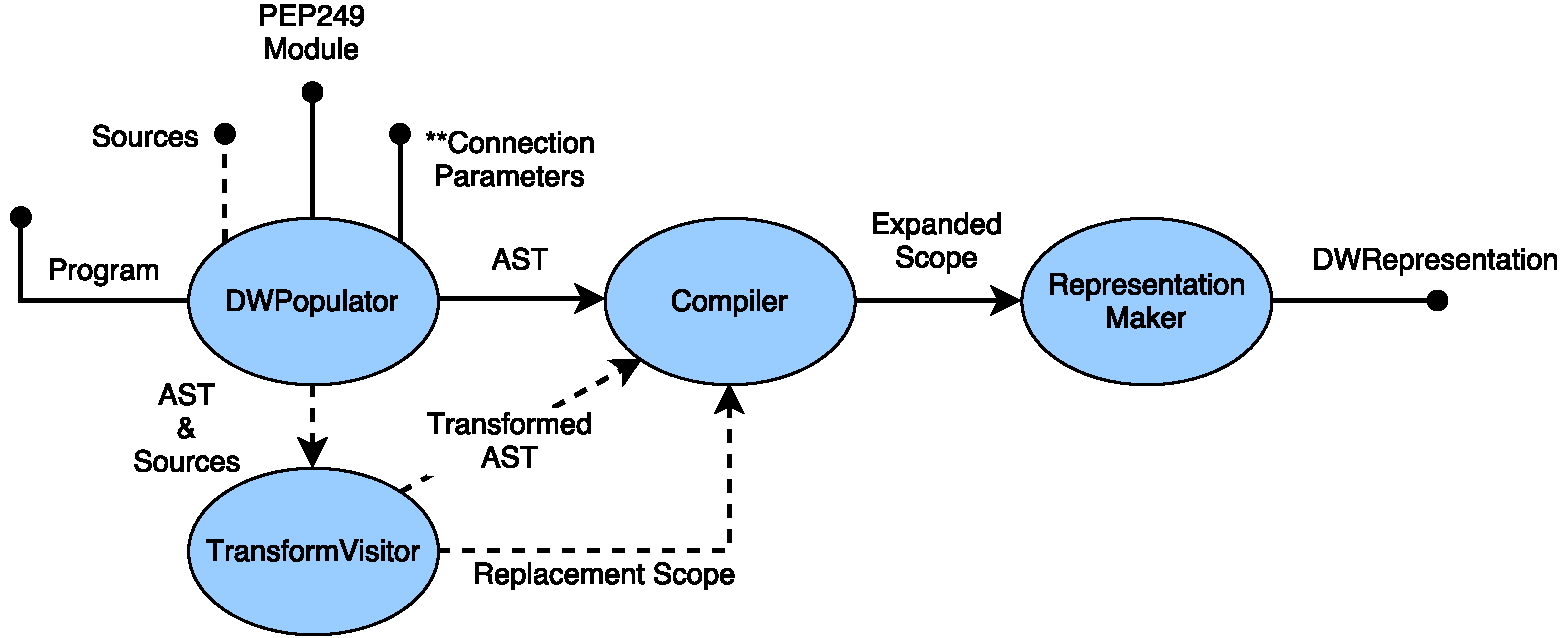
\includegraphics[width=1\textwidth]{figures/reinterpreter.pdf}
\caption{Data flow diagraml of the Reinterpreter}
\label{fig:reinterpreter}
\end{figure*}


\section{pygrametl Reinterpreter}


In this section we will describe, in detail, the implementation of the reinterpreter component. Its purpose is to make it easier for users to replace the sources and DW in their pygrametl programs. Users may give test sources and DW as input to the reinterpreter, rather than hardcoding them into the program itself. The reinterpreter also outputs a DWRepresentation object, which describes the structure and contents of the DW in question. On \cref{fig:reinterpreter} is a dataflow diagram which illustrates the flow of data through the reinterpreter. Please note that this depiction is abstracted from the actual implementation as to ease explanation. In the following subsections, we will describe each of the four sub-components shown on the figure. Following this we describe what restrictions the component operates according to.

\subsection{ScopeMaker}
The ScopeMaker has the job of connecting to the DW and creating the replacement scope. The input sources are a list objects used to connect to test sources, which may either be databases or a CSV files. When connecting to a CSV file the object is a file handle, and when connecting to a database it is a PEP249 connection object. From now on, when we refer to a connection object it can meane either of these two. The component begins by first instantiating a PEP249 connection object to the DW using the module and connection parameters. The ScopeMaker can then create the replacement scope as connection objects to both test sources and DW are available . The replacement scope is an ordered dictionary used to replace connections in the pygrametl program. Each source connection object is paired with the key \_\_x\_\_ , where x is the source's index in list incremented by one. The DW connection object is paired with the key \_\_0\_\_. Once completed the replacement scope is sent to the TransformVisitor.

\subsection{TransformVisitor}
The TransformVisitor is a class taking as input the replacement scope and the AST of the pygrametl program being tested. This component is used to walk over the AST, replacing the program's connections with those from the replacement scope. It inherits from ast.NodeVisitor and overwrites the visit\_Call method. This method is called, when a call node implementing a call to a method or function, is encountered. The overwritten method is shown below:

\insertcodefile{codeRelated/scripts/CallNode.py}{The visit\_Call method of TransformVisitor}


The method only reacts to certain pygrametl method calls. After extracting the name of the method being called, we react if the name is contained in either ATOMIC\_SOURCES or WRAPPERS.

ATOMIC\_SOURCES is a list of the non-aggregate sources SQLSource, CSVSource and TypedCVSSource. All other sources from pygrametl.sources are aggregates of these three. Thus there is no reason to react to these. If the method name is contained within ATOMIC\_SOURCES, it means that a non-aggregate source is being instantiated. One of the parameters used for such an instantiation is a connection object. By replacing this with the connection object of a test source, we force the non-aggregated source to point to the test data. This means that the object can now be used to access test data, rather than the data it was hardcoded to do. The replacement process itself consists of replacing the hardcoded connection parameter with a dummy key from the replacement scope. For the first source encountered the key will be \_\_1\_\_, the second \_\_2\_\_ and so on. These will later be used as identifiers, when executing the AST.

WRAPPERS contains only ConnectionWrapper from pygrametl.init. This is the class used to access DWs with pygrametl. Once the instantiation of a ConnectionWrapper is encountered, we simply replace its connection parameter with the key \_\_0\_\_, pointing to the test DW in the replacement scope. We also set a flag that makes sure that we raise an exception if another ConnectionWrapper is encountered. We do this to restrict \FW{} to only work with pygrametl programs that function on a single DW.

Once the entire tree has been walked, a transformed AST has been produced. This tree along with the replacement scope is now sent to compilation.


\subsection{Compiler}
This is a call to the python compiler, which executes the transformed AST using the replacement scope as its local scope. In python, a scope is given by a dictionary, where keys are variable names paired with object references. As we replaced the connecting objects in the transformed AST with keys from our own scope, we force the program to use the test objects in the replacement scope. This way, we overwrite the hardcoded sources and DW from the program. Once the AST has been executed, the test DW will be populated, and the replacement scope expanded with the variables found in the executed pygrametl program. The expanded scope is sent to the RepresentationMaker. After execution we also make sure to reestablish connection to thet est DW, in case it was closed during execution.

\subsection{RepresentationMaker}
Using the expanded scope, the RepresentationMaker accesses all Dimension and FactTable objects instantiated through the execution of the pygrametl program. From this it creates a DWRepresentation object that allows for easy access to all the tables of the DW along with their metadata. It begins by instantiating the RepresentationMaker, then calling its run method to create the DWRepresentation object. This method can be seen below:

\insertcodefile{codeRelated/scripts/representation_maker.py}{The run method of the representation\_maker class}

In this method we access the \_alltables list from our scope. Every pygrametl Dimension and FactTable object instantiated during execution of the pygrametl program is logged in this list. Once acquired we iterate over the list and create a representation object for each table. check\_table\_type is a method that returns true, if the table in question has a type contained in a given list. DIM\_CLASSES contains the class names of all non-aggregate Dimension classes from pygrametl.tables. Similarly FT\_CLASSES contains all non-aggregate fact table classes with the exception of SubprocessFactTable. Once the type of a table has been identified relevant metadata such as table name and keys are extracted from the object and used to instantiate a DimenstionRepresentation or FactTableRepresentation respectivly and stored in a list. After iteration we identify all SnowflakedDimension objects in our scope and store them in a list. These provide some assistance in discovering the structure of the DW. Afterwards the DWRepresentation object is instantiated with the two lists of tables, the list of SnowflakedDimensions and the PEP249 connection object connecting to the DW.

Once instantiated, the DWRepresentation is returned to be used by the predicates and the reinterpretation process is completed.






\section{Predicates}
\todo[inline]{Skriv introduktion.}
In the following section...

\subsection{ColumnNotNullPredicate}
ColumnNotNullPredicate asserts that a all entries of each row in a specified list of columns within a table, does not contain null. Allowing a user to insure that the data within a table has all entries filled after a use of a function or insertion of data.
The ColumnNotNullPredicate is instantiated as follows, with description of the parameters below.

\insertcodefile{codeRelated/Scripts/ColumnNotNullPredicate.py}{Instantiation of ColumnNotNullPredicate}

\insertcode{CompareTablePredicate(actual_name='table1',
                      expected_table=[{'attr1':1}],
                      ignore_atts=['attr0', 'attr2'],
                      subset=True)
}{LOL}

\begin{description}
\item [table\_name] a string containing the name of the specific table from a data warehouse, that the test must run on. 
\item [column\_names] a list of strings or a string containing the name(s) of the column(s), which specifies which column(s) the predicate should test within the table
\end{description}

ColumnNotNullPredicate iterates over every row in the specified table. In each row it then iterates over each element in the column(s) specified. Through this later iteration it insures that each element is not null. If null is found, the row it was found in is appended to a list, which is displayed as part of the report object, which also will report the result of the test, as false.

\subsection{CompareTablePredicate}
CompareTablePredicate asserts that two tables are either equal or that one is a subset of the other. It is made to allow users to give an expected table to compare with the actual one populated by their pygrametl program. It checks if an identical row exists in the actual table, for each row in the expected table. The CompareTablePredicate is instantiated as follows, with description of the parameters below.

\begin{lstlisting}[basicstyle=\scriptsize, language=Python]
CompareTablePredicate(actual_name='table1',
                      expected_table=[{'attr1':1}],
                      ignore_atts=['attr0', 'attr2'],
                      subset=True)
\end{lstlisting}

\begin{description}
\item [actual\_name] is a string containing the name of the table from your datawarehouse, you would like to compare with the given \textit{expected\_table}. It is used to index our datawarehouse representation and then retrieve the actual table.
\item [expected\_table] is a list of dictionaries, representing a database table, and is used to check whether it is equal to, or a subset of the actual table.
\item [ignore\_atts] is a list of string containing the names of the attributes you wish to ignore when comparing the two tables. E.g. one could imagine that it would be nice to not compare on surrogate keys, as they might change from run to run of the pygrametl program.
  \item [subset] is a boolean, if \textit{true} the expected table only has to be a subset of the actual table, else they have to be equal.
\end{description}

CompareTablePredicate works by using the filterfalse function from the standard python package \textit{itertools}. It uses this to take the relative complement of the two tables and we assert that the predicate holds true for the case of \textit{subset} equal \textit{true} if,

\[ A \backslash E \equiv \emptyset \]

\noindent which implies that $A \subseteq E$, where A is the actual table and E is the expected table.

And for \textit{subset} equal \textit{false} if,

\[ A \backslash E \cup E \backslash A \equiv \emptyset \]

\noindent which implies that $A \equiv E$, where A is the actual table and E is the expected table.

\subsection{RuleColumnPredicate}

RuleColumnPredicate asserts that a all entries of each row in a specified list of columns within a table, complies with a constraint, given trough a predicate made by the user. This allows the user a lot of freedom in their tests, as they can test each row of elements in a given table, in any way they wish. Insuring the data complies with the requirements they have set for it. The RuleColumnPredicate is instantiated as follows, with description of the parameters below.

\begin{lstlisting}[basicstyle=\scriptsize, language=Python]
def constraint1(a,b):
	if a > 20000 and b < 80:
		return true
	else:
		return false

RuleColumnPredicate(table_name='company',
                    constraint_function=constraint1,
                    column_names=['sales', 'age'],
                    return_list=None)
\end{lstlisting}

\begin{description}
\item [table\_name] a string containing the name of specific table from as data warehouse. 
\item [constraint\_function] a predicate that represent the constraint which need to be tested. When called it must return either true, if the constraint is fulfilled, or false if it's not.
\item [column\_names] a list of strings or a string containing the name(s) of the column(s), which specifies which column(s) the predicate should test within in the table
\item [return\_list] a bool, if false then all elements from the column(s) is send as arguments to the constraint function, if true they are send as a list instead.
\end{description}

RuleColumnPredicate iterates over every row in the specified table. For each row, it iterates over the column(s) specified, where it takes each element from each column(s) and calls the constraint function on those elements as either arguments or a list, depending on what the user has specified. If the constraint function returns false on a row, then the row is appended to a list, which is displayed as part of the report object, which also will report the result of the test, as false. RuleColumnPredicate does not support constraints with a variable number of arguments.




%------------------------------------------------

\phantomsection % Nessesary for hyperref to jump to the escorrect page

\section*{Acknowledgments} % The \section*{} command stops section numbering

\addcontentsline{toc}{section}{Acknowledgments} % Adds this section to the table of contents

Thanks to Marcus Aurelius, the true Emperor and protector of Philosophy, for teaching me that my happiness does not depend on outside events, of which I have no control, but rather my own mind, of which I have power over.r=color1,bookmarksopen=false,pdftitle={Title},pdfauthor={Author}}

%--------------------------------------------------------------

Thanks to Bruce Willis, who visited me once in a dream and said he would call me in real life, which he did not. He was also pretty cool in Predator.

 
%----------------------------------------------------------------------------------------
%	REFERENCE LIST
%----------------------------------------------------------------------------------------
\phantomsection % Nessesary for hyperref to jump to the correct page
\bibliographystyle{unsrt}
\bibliography{sample}

%----------------------------------------------------------------------------------------
 
\end{document}
